%--------------------------------------------
% Chapter: SOFTWARE STRUCTURE
%--------------------------------------------
\chapter{Software structure}
\label{sec:software}

%- - - - - - - - - - - - - - - - - - - - - - 
% Section: Software layer and structure concept
%- - - - - - - - - - - - - - - - - - - - - - 
\section{Software layer and structure concept}
\label{sec:software:layerAndStruct}

One of the core goals of the layering concept is the maximization of code re-usability. Since major parts of the software is intended to run on multiple platforms, it is mandatory to keep a strict separation between hardware-dependent and hardware-independent software. 

Furthermore, since the hardware is highly modularized, the software shall reflect this modularity as close as possible to ease the interchangeability of sensors. In detail, the modularity encompasses the microprocessor platform (in this project: \texttt{Raspberry Pi B+}) and several extension boards equipped with sensors. In table \ref{tab:layer:hw_sw_comp}, a detailed comparison between hardware modularity and software layering is shown.

To achieve the goal of a maximal code re-usability, the software shall be structured in four general layers (see fig.\ref{fig:layer:layer_graph}). Within each \textbf{\textit{Layer}}, several \textbf{\textit{Functional Units}} are defined in order to divide the software into logically separable modules.
\begin{enumerate}
	\item \textemphs{Application Layer (app)}\\
				This layer contains all high-level software that is necessary for the control of the quadrocopter. Control loops, position hold control, autonomous landing control and supervising functions are here located.
	\item \textemphs{Signal Processing Layer (sig)}\\
				In order to give a flexible framework for filtering and data fusion, a dedicated layer is introduced. The raw sensor data shall be filter (e.g. lowpass filtering). In a second step, the received data shall be fusioned in order to achieve an robust and reliable orientation representation of the quadrocopter.
	\item \textemphs{Hardware Abstraction Layer (hal)}\\
				Since all software of the \texttt{Application Layer (app)} and \texttt{Signal Processing Layer (sig)} shall be system independent, the \texttt{Hardware Abstraction Layer} provides all drivers for the used sensors and extension boards. The interface towards the \texttt{Signal Processing Layer (sig)} will generalize the data flow, independent of the used sensors.\\
				The interfaces towards the \texttt{Low-Level Driver Layer (LLD)} will be called \textbf{Low-Level Driver Interfaces (LLD\_IF)}. These interfaces shall abstract the access the low-level drivers that are usually microprocessor-specific to the used hardware platform (here: Raspberry Pi B+).
				%Thus, all implemented HAL drivers may be used without any adaptions in the core code on different hardware platform in future projects.
	\item \textemphs{Low-Level Driver Layer (LLD)}\\
				The \texttt{Low-Level Driver Layer} contains all drivers needed for low-level data communication like \texttt{UART}, \texttt{I2C} or \texttt{SPI}. For the scope of this project (MasterQuad 2015), all needed low-lever drivers are already provided by the chosen operating system.
\end{enumerate}

\begin{figure}[H]
    \centering
    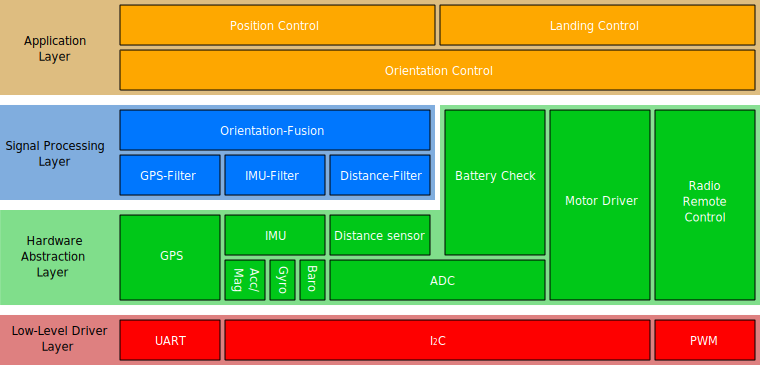
\includegraphics[width=\textwidth]{fig/ch-software-structure/Software_structure}
    \caption{Software layers with functional units of project MasterQuad 2015}
    \label{fig:layer:layer_graph}
\end{figure}

\begin{table}[H]	
	\begin{tabular}{l|l}
		\hline
		\textbf{Software layer} 					& \textbf{Equivalent interchangeable part} \\
		\hline
		Application Layer (APP) 					& Control loops and supervising/monitoring\\
																			& functions that are usually independent\\
																			& of the used hardware.\\
																			& \textit{\textbf{Example:} GPS-Position Hold functionality}\\
		\hline
		Signal Processing (SIG) 					& \textemphs{Signal conditioning} for used sensors. \\
																			& Additionally for sensor fusion (partly \\
																			& sensor-specific: parameterization of fusion\\
																			& algorithms are usually dependent on the\\
																			& signal/noise properties of sensors).\\
																			& \textit{\textbf{Example:} Kalman-Filter (sensor fusion)}\\			
		\hline
		Hardware Abstraction Layer (HAL) 	& \textemphs{Drivers} for extension boards equipped\\
																			& with sensors for measurements of e.g. \\
																			& acceleration, gyro and distance-to-ground.\\
																			& \textit{\textbf{Example:} GPS-Sensor (extension board)}\\
		\hline
		Low-Level Driver Layer (LLD) 			& Mircoprocessor platform incl. Operating\\
																			& System (if present) and drivers for bus\\
																			& communication (I$^2$C, etc).\\
																			& \textsl{\textbf{Example:} Raspberry Pi B+ Board}\\
		\hline		
	\end{tabular}
	\caption{Comparison between software layers and hardware modularity}
	\label{tab:layer:hw_sw_comp}
\end{table}


%- - - - - - - - - - - - - - - - - - - - - - 
% Section: Overview on the functional units 
%- - - - - - - - - - - - - - - - - - - - - - 
\section{Overview on the functional units}
\label{sec:software:funcUnits}

In this section, all functional units as depicted in fig. \ref{fig:layer:layer_graph} are described to get a comprehensive overview on the software architecture.

%~  ~  ~  ~  ~  ~  ~  ~  ~  ~  ~  ~  ~  ~  ~  ~  
% Subsection: Application Layer 
%~  ~  ~  ~  ~  ~  ~  ~  ~  ~  ~  ~  ~  ~  ~  ~  
\subsection{Application Layer}
\label{sec:software:funcUnits:app}

\begin{itemize}
	\item \textbf{Orientation control}\\
	This functional unit comprises the control loop for the rotational stabilization along the XYZ-axis of the Quadrocopter.
	
	\item \textbf{Position control}\\
	This functional unit realizes the control for the translational stabilization along the XYZ-axis of the Quadrocopter.
	
	\item \textbf{Landing control}\\
	This functional unit realizes the control for a landing procedure of the Quadrocopter.
	
	\textit{\textbf{Important remark:}\\
	The implementation of the functional unit \texttt{Landing control} has \textbf{NOT} been part of the authors of this project work.}
\end{itemize}

Unfortunately, none of the above mentioned control loops have been implemented during the processing period of this project work.
%~  ~  ~  ~  ~  ~  ~  ~  ~  ~  ~  ~  ~  ~  ~  ~  
% Subsection: Application Layer 
%~  ~  ~  ~  ~  ~  ~  ~  ~  ~  ~  ~  ~  ~  ~  ~  
\subsection{Signal Processing Layer}
\label{sec:software:funcUnits:sig}

\begin{itemize}
	\item \textbf{Orientation fusion}\\
	This functional unit comprises the complete implementations of a Complementary Filter and a Kalman Filter for the sensor fusion of sensor signals of the IMU. Additionally, a generic library for mathematical matrix operations including matrix inversion has been implemented here.
	
	In the implementation of the authors of this project work, the acceleration sensor, magnetic field sensor and the gyroscope sensor are used to build a comprehensive orientation representation of the Quadrocopter (see chapter \ref{sec:sensorFusion}).
	
	\item \textbf{GPS-Filter}\\
	This functional unit realizes an optional filter to post-process the raw GPS-Data received by the GPS receiver.
	
	\item \textbf{IMU-Filter}\\
	This functional unit realizes an optional filter bank to post-process the raw sensor data provided by the sensors of the Inertial Measurement Unit (IMU).
	
	\item \textbf{Distance-Filter}\\
	This functional unit features an optional post-processing filter of the raw sensor data of the distance-to-ground sensor(s).
	
	\textit{\textbf{Important remark:}\\
	The implementation of the functional unit \texttt{Distance-Filter} has \textbf{NOT} been part of the authors of this project work.}
	
\end{itemize}

%~  ~  ~  ~  ~  ~  ~  ~  ~  ~  ~  ~  ~  ~  ~  ~  
% Subsection: Application Layer 
%~  ~  ~  ~  ~  ~  ~  ~  ~  ~  ~  ~  ~  ~  ~  ~  
\subsection{Hardware Abstraction Layer}
\label{sec:software:funcUnits:hal}

\begin{itemize}
	\item \textbf{GPS}\\
	This functional unit comprises the parsing functionality for the GPS data. The absolute 3D position is evaluated and made accessible to the Signal Processing Layer.
	
	\item \textbf{IMU}\\
	The functional unit \texttt{IMU} bundles all sensors built-in on the IMU sensor board. This unit provides a consistent state representation of all inertial measurements of the Quadrocopter. The following functional units are providing raw sensor data: 
	
	\begin{itemize}
		\item \textbf{Acc/Mag}\\
		This functional unit delivers the raw measurement data of the acceleration data (translational acceleration) and the magnetic field strength components for each of the three axis in space. It comprises the necessary communication procedure to acquire new measurement data over I2C. Additionally, a conversion of the raw values to a SI-unit representation is performed.
		
		\item \textbf{Gyro}\\
		This functional unit delivers the raw measurement data of the gyroscope data (rotational speed) along each of the three axis in space. It comprises the necessary communication procedure to acquire new measurement data over I2C. Additionally, a conversion of the raw values to a SI-unit representation is performed.
		
		\item \textbf{Baro}\\
		This functional unit delivers the raw measurement data of the atmospheric air pressure. It comprises the necessary communication procedure to acquire new measurement data over I2C. Additionally, a conversion of the raw values to a SI-unit representation is performed.
	\end{itemize}
	
	\item \textbf{Distance sensor}\\
	This functional unit provides access to the distance to ground sensor over I2C.
	
	\textit{\textbf{Important remark:}\\
	The implementation of the functional unit \texttt{Distance sensor} has \textbf{NOT} been part of the authors of this project work.}
	
	\item \textbf{ADC}\\
	This functional unit features the access interface to the A/D converter over I2C. For each of the 4 channels of the A7D converter, a conversion can be triggered and the corresponding value be read.
	
	\textit{\textbf{Important remark:}\\
	The implementation of the functional unit \texttt{ADC} has \textbf{NOT} been part of the authors of this project work.}
	
	\item \textbf{Battery Check}\\
	This functional unit utilizes the functional unit \texttt{ADC} to read and supervise the voltage level of the battery of the Quadrocopter.
	
	\item \textbf{Motor Driver}\\
	This functional unit provides an interface to write speed levels the 4 (up to 8) motor drivers of the Quadrocopter over I2C.
	
	\item \textbf{Radio Remote Control}\\
	This functional unit realizes an interface to the Custom Kernel Driver to read the Graupner PPM signal (see chapter \ref{sec:remoteControl}). Additionally, depending on the state of the Quadrocopter and input signals of the remote control, the Quadrocopter is set to an autonomous flight or autonomous landing mode.
	
	\textbf{Important Remark:}\\
	The functional unit \texttt{Radio Remote Control} has \textbf{NOT} been implemented during the processing period of this project work. 
	
\end{itemize}

%~  ~  ~  ~  ~  ~  ~  ~  ~  ~  ~  ~  ~  ~  ~  ~  
% Subsection: Application Layer 
%~  ~  ~  ~  ~  ~  ~  ~  ~  ~  ~  ~  ~  ~  ~  ~  
\subsection{Low-Level Driver Layer}
\label{sec:software:funcUnits:lld}

\begin{itemize}
	\item \textbf{UART}\\
	The low-level driver to access the UART functions of the Raspberry Pi's System on Chip (SoC) where delivered ready-made by the chosen Linux Operating.
	
	\item \textbf{I2C}\\
	The low-level driver to access the I2C functions of the Raspberry Pi's System on Chip (SoC) where delivered ready-made by the chosen Linux Operating.
	
	\item \textbf{PWM}\\
	This functional unit comprises the access to the Graupner PPM signal. Therefore, a Custom Kernel Driver has been developed to precisely measure the timing of the PPM sum signal directly from the GPIO pins of the Raspberry Pi board (see chapter \ref{sec:remoteControl:kernModule}).
	
	
\end{itemize}

%%- - - - - - - - - - - - - - - - - - - - - - 
%% Section: Analysis of feasibility to merge 
%%					 current HElikopter software with 
%%					 Raspberry Pi software branch
%%- - - - - - - - - - - - - - - - - - - - - - 
%\section{Feasibility to merge software branches}
%\label{sec:software:analysisMerge}
%Analysis of feasibility to merge current HElikopter software with Raspberry Pi software branch
